\documentclass{beamer} % [handout] para imprimir eliminando transiciones

%\usefonttheme[onlymath]{serif}
%\usepackage{fontspec}
%\defaultfontfeatures{Mapping=tex-text}
%\setsansfont[Ligatures={Common}]{Futura}
%\setmonofont[Scale=0.8]{Monaco}

\usepackage{beamerthemesplit}
\usepackage[utf8]{inputenc}
\usepackage[spanish]{babel}
\mode<presentation>
\usetheme{default}
\usecolortheme{dolphin}
\usepackage{alltt}    % \begin{alltt}
\usepackage{amssymb}  % mathematical symbols
\usepackage{comment}
\usepackage{multicol} % \multicols
\usepackage{multirow} % \multirows
\usepackage{tabto}    % \tabto
\usepackage{verbatim} % comentarios

\title{Estructuras de datos}   %[titulo corto]
\author{Fabián Riquelme Csori} %[nombre corto]
\date{2017}                    %[fecha corta]
\institute{Universidad de Valparaíso}                 %[instituto corto]

\newcommand{\HRule}{\rule{\linewidth}{0.2mm}\\[1ex]}
\newcommand{\blue}[1]{\textcolor{blue}{#1}}
\newcommand{\red}[1]{\textcolor{red}{#1}}
\newcommand{\redb}[1]{{\color{red!70!black}{#1}}}
\newcommand{\green}[1]{{\color{green!70!black}{#1}}}
\newcommand{\gray}[1]{{\color{gray!50!white}{#1}}}
\newcommand{\textgreek}[1]{\begingroup\fontencoding{LGR}\selectfont#1\endgroup}
% \alert{texto destacado en rojo}
% \color{green} Color en verde
% \structure{texto en lila}

\begin{document}


%\begin{frame}%[plain]
%  \titlepage
%\end{frame}
%
% [opciones]:
% plain: oculta barra de navegacion, deja + espacio para contenido
% fragile: usar comandos como verbatim
% b,c,t: alineacion vertical
% label=nombre_etiqueta
% allowframebreaks: divide contenido en varios frames si es demasiado largo
% shrink: para escribir mucho texto en una transparencia, reduciendo tamano de fuente

%%%%%%%%%% PORTADA %%%%%%%%%%
\begin{frame}[plain]
  \begin{figure}[h]
    \begin{minipage}{0.3\textwidth}
    
\includegraphics[width=.9\textwidth]{./image/logo-UV.png}
    \end{minipage}
    \begin{minipage}{0.65\textwidth}
     $~$\\[3.6ex]
     \footnotesize{Escuela de Ingeniería Civil Informática}\\
     \footnotesize{Facultad de Ingeniería}
    \end{minipage}
  \end{figure}
  \begin{center}
    \vspace{1ex}
    \HRule
    \Large{Estructuras de datos}\\{\small Capítulo V: Algoritmos de ordenamiento}\\[-1ex]
    \HRule\vspace{1ex}
    \large{Fabián Riquelme Csori}\\[.5ex]\footnotesize{fabian.riquelme@uv.cl}\\[6ex] {\tiny 2017-II}\\[6ex]
  \end{center}
\end{frame}

%%%%%%%%%% INDEX %%%%%%%%%%
\begin{frame}
 \frametitle{Index}
 \scriptsize 			% reducir tamano de letra
 \tableofcontents		%[pausesections]
\end{frame}

%%%%%%%%%%% ACTUAL INDEX %%%%%%%%%%
%\AtBeginSection[] %generar indice automaticamente
%{
%\begin{frame}<beamer>%[plain]
% \frametitle{Index}
% \framesubtitle{subtitulo}
% \scriptsize
% \tableofcontents[currentsection, currentsubsection]
%\end{frame}
%}

%==============================
\section{Problemas de ordenamiento}

%-----------------------
\subsection{Fundamentos}



\begin{frame}{Aplicaciones}
    \begin{itemize}
        \item Compresión de datos
        \item Computación gráfica
        \item Planificación de tareas
        \item Balanceado de carga en computación paralela
        \item Bioinformática
        \item Simulación (sistemas de partículas)
        \item Gestión de cadenas de suministro
        \item Sistemas de recomendaciones
        \item etc. etc. etc.
    \end{itemize}
\end{frame}

%==============================
\section{Algoritmos de ordenamiento}

%-----------------------
\subsection{Algoritmos básicos}

\begin{frame}{Ordenamiento por inserción}
    \begin{itemize}
        \item {\footnotesize En cada iteración, se inserta un elemento del subvector no ordenado en la posición correcta dentro del subvector ordenado.}
    \end{itemize}
    \begin{center}
        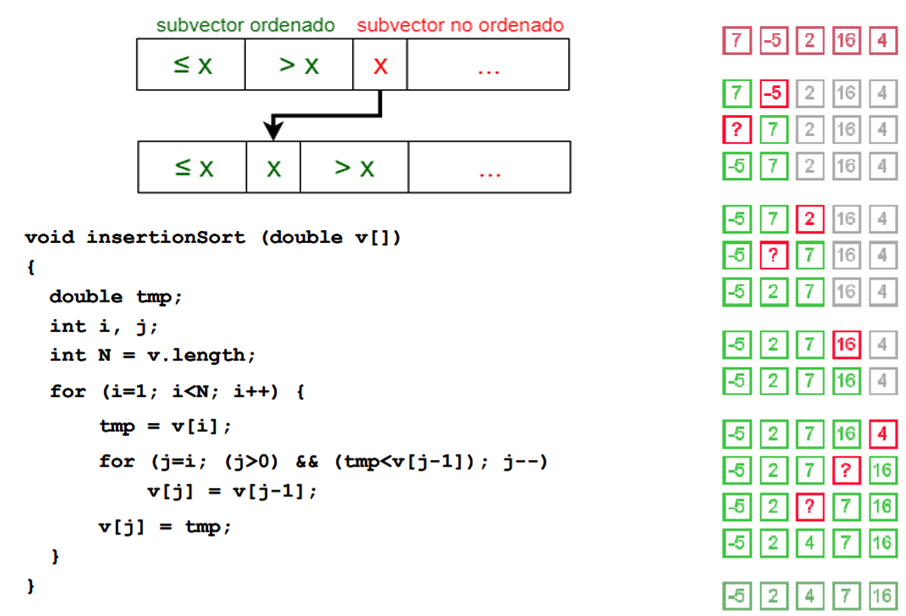
\includegraphics[width=.8\textwidth]{./image/cap5/insertion-sort.png}
    \end{center}
\end{frame}

\begin{frame}{Ordenamiento por selección}
    \begin{itemize}
        \item {\footnotesize En cada iteración, se intercambia el menor elemento del subvector no ordenado con el primer elemento de dicho subvector.}
    \end{itemize}
    \begin{center}
        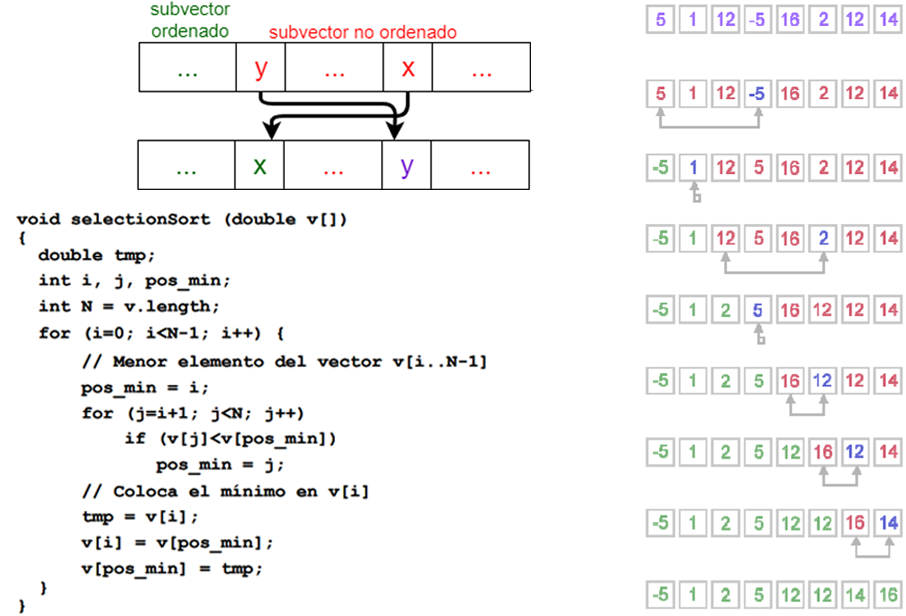
\includegraphics[width=.8\textwidth]{./image/cap5/selection-sort.png}
    \end{center}
\end{frame}

\begin{frame}{Ordenamiento de burbuja}
    \begin{itemize}
        \item {\footnotesize En cada iteración se compara cada elemento con el siguiente, intercambiándolos de posición si están en el orden equivocado.\\
        El proceso se repite tantas veces como sea necesario.}
    \end{itemize}
    \begin{center}
        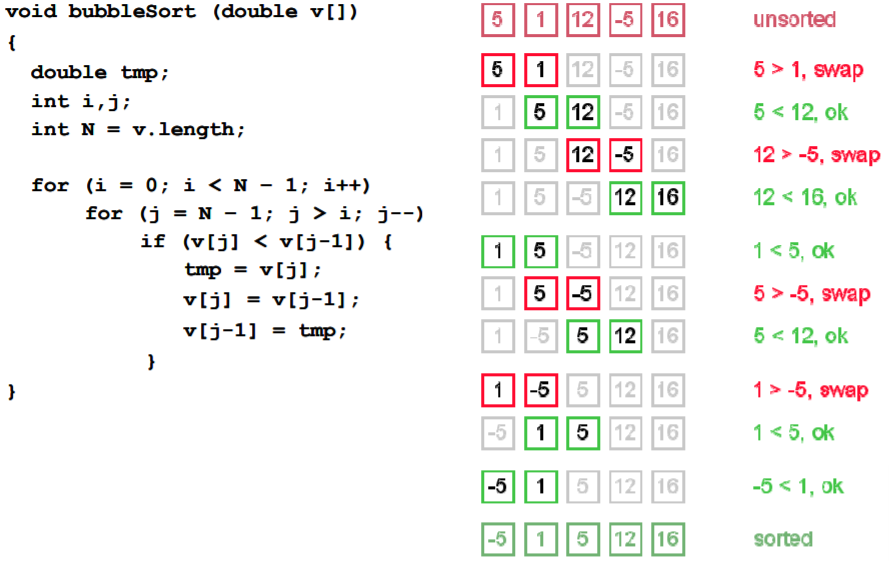
\includegraphics[width=.8\textwidth]{./image/cap5/bubble-sort.png}
    \end{center}
\end{frame}

\begin{frame}{Ordenamiento de burbuja (centinela)}
    \begin{itemize}
        \item {\footnotesize Este algoritmo se puede mejorar para cuando el vector está casi ordenado. Mediante un centinela se termina cuando en una iteración del bucle interno no se produce intercambio.}
    \end{itemize}
    \begin{center}
        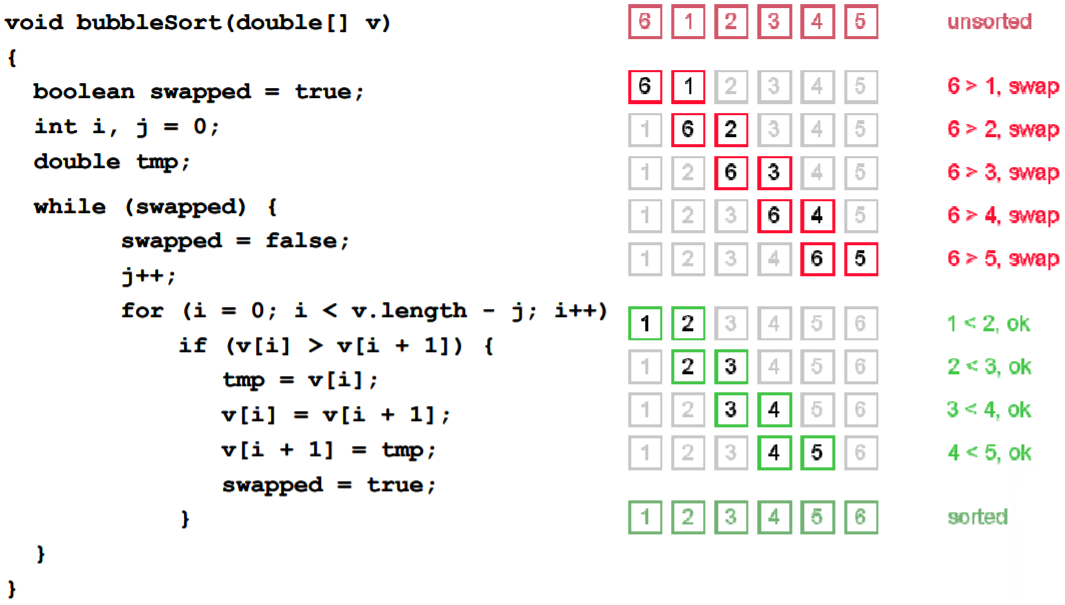
\includegraphics[width=.9\textwidth]{./image/cap5/bubble-sort2.png}
    \end{center}
\end{frame}

\begin{frame}{Ejercicios}
    \begin{itemize}
        \item Ordenar ``en papel'' el siguiente vector utilizando los tres métodos anteriores: \blue{[8, 5, 2, 6, 9, 3, 1, 4, 0, 7]}.
      %  \item Implementar los pseudocódigos anteriores y comprobar sus resultados del ejercicio anterior.
    %    \item Incluir un contador de iteraciones en sus algoritmos y comprobar cuál requiere menos iteraciones de los tres.
    \end{itemize}
\end{frame}

%-----------------------
\subsection{Algoritmos más eficientes}

\begin{frame}{Ordenamiento por mezcla ({\em Merge sort})}
    \begin{itemize}
        \item {\footnotesize Usa la estrategia \blue{divide y vencerás}. Se divide el vector en dos mitades;\\ se ordena recursivamente cada mitad (usando el mismo método),\\ y se van combinando las dos mitades ordenadas.}
    \end{itemize}
    \begin{center}
        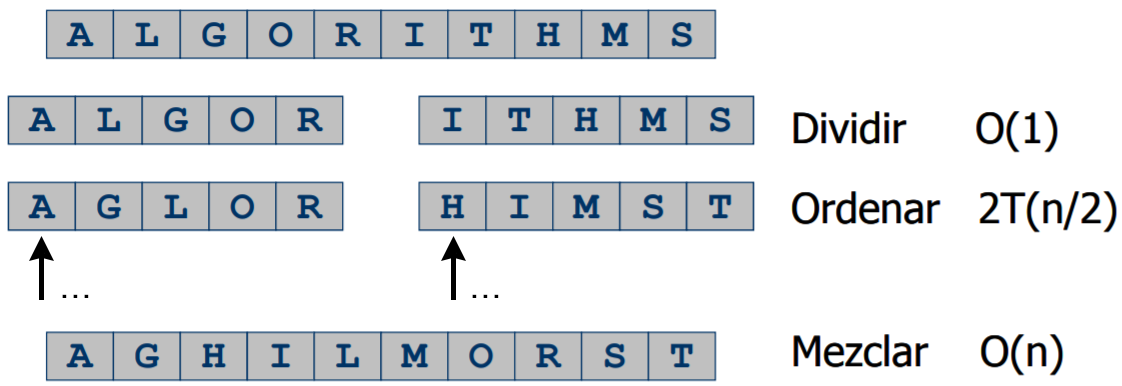
\includegraphics[width=.9\textwidth]{./image/cap5/merge-sort1.png}
    \end{center}
\end{frame}

%FRC aqui se explica la complejidad:
%http://elvex.ugr.es/decsai/algorithms/slides/problems/Sorting.pdf

\begin{frame}{Ordenamiento por mezcla ({\em Merge sort})}
    \begin{center}
        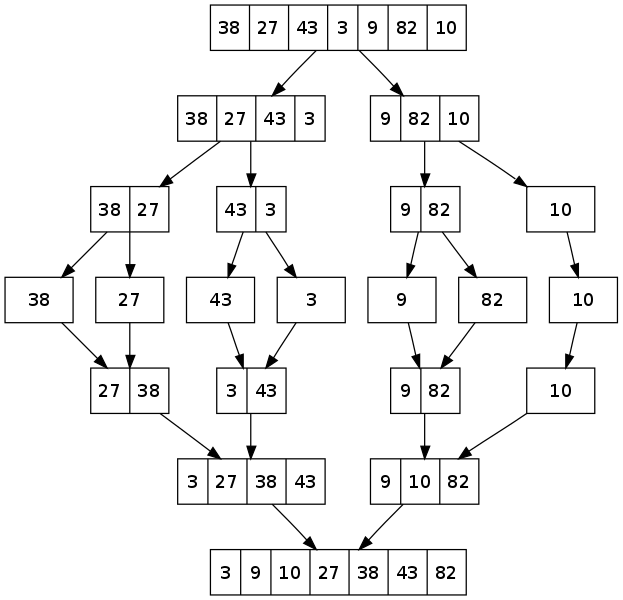
\includegraphics[width=.65\textwidth]{./image/cap5/merge-sort2.png}
    \end{center}
\end{frame}

\begin{frame}{Ordenamiento rápido ({\em Quicksort})}
    \begin{itemize}
        \item Se toma un elemento arbitrario del vector (\blue{pivote} $p$). El vector se \blue{particiona} tal que a izquierda queda todo $\leq p$ y a derecha $\geq p$. Se ordena por separado cada zona delimitada por pivote.
        \vspace{2ex}

        \begin{center}
            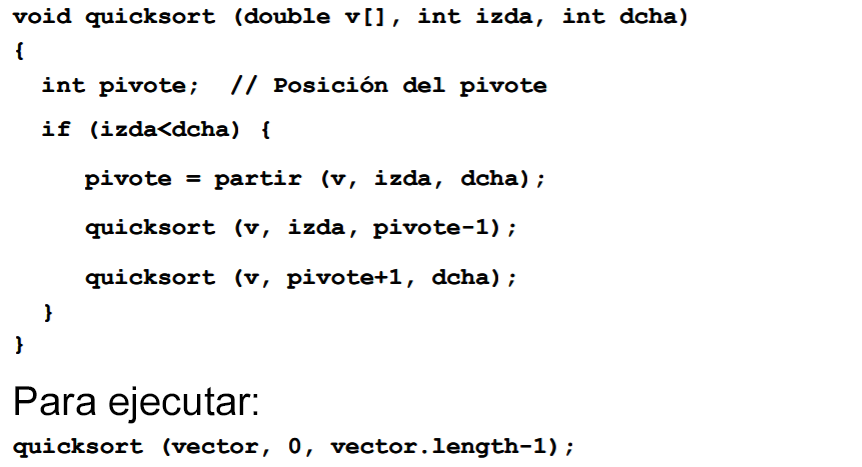
\includegraphics[width=.85\textwidth]{./image/cap5/quicksort1.png}
        \end{center}
    \end{itemize}
\end{frame}

\begin{frame}{Ordenamiento rápido ({\em Quicksort})}
    \begin{minipage}{0.51\textwidth}
    {\small Para la partición:
    \begin{itemize}
        \item Recorrer el vector de izq a der hasta encontrar un elemento en posición $i$ tal que $v[i]>p$.
        \item Recorrer el vector de der a izq hasta encontrar un elemento en posición $j$ tal que $v[j]<p$.
        \item Intercambiar los elementos ubicados en $i$ y $j$, de modo que $v[i]<p<v[j]$.
    \end{itemize}}
    \end{minipage}
    \begin{minipage}{0.47\textwidth}
        \begin{center}
            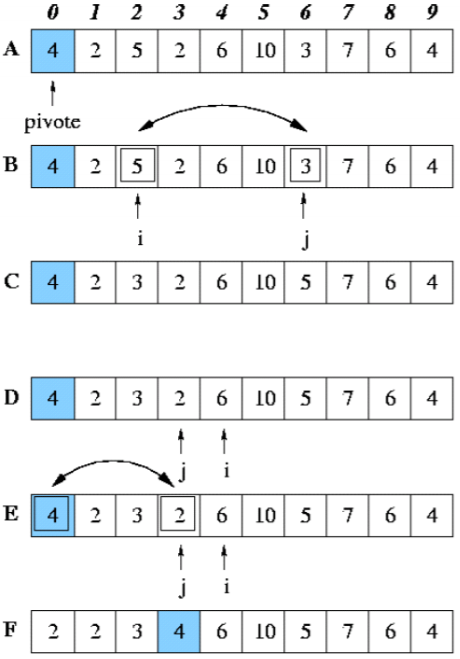
\includegraphics[width=.9\textwidth]{./image/cap5/quicksort2.png}
        \end{center}
    \end{minipage}
\end{frame}

\begin{frame}{Ordenamiento rápido ({\em Quicksort})}
    \begin{center}
        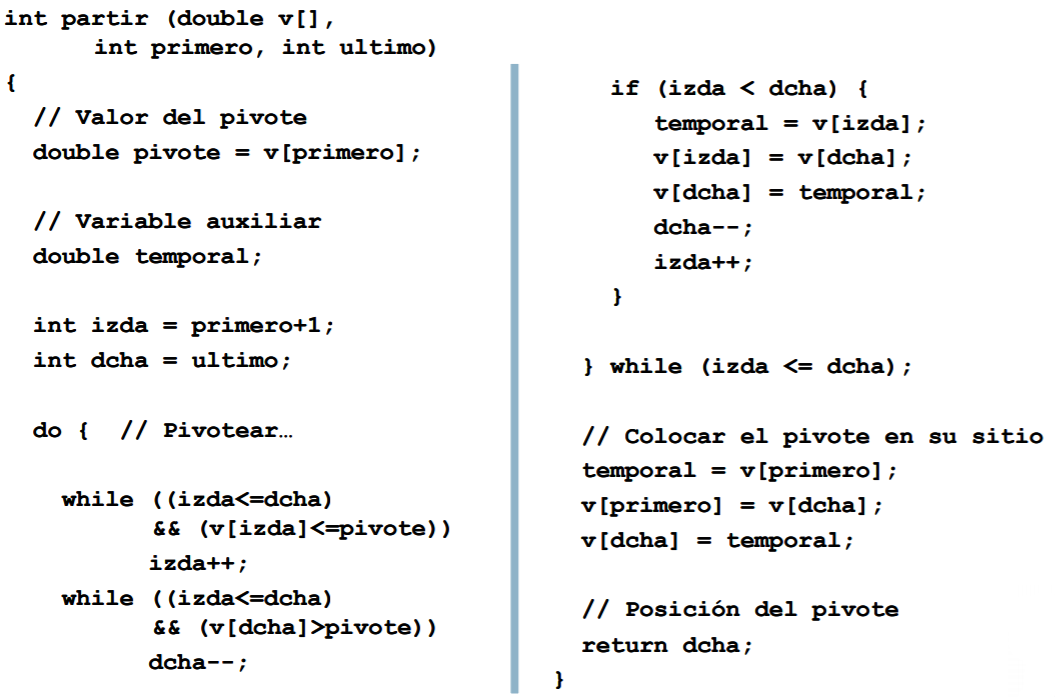
\includegraphics[width=.9\textwidth]{./image/cap5/quicksort3.png}\\
        {\scriptsize Para conjuntos grandes es conveniente elegir el pivote en el medio.}
    \end{center}
\end{frame}

\begin{frame}{Mejoras del ordenamiento de inserción}
    \begin{itemize}
        \item \blue{Heapsort} o \blue{algoritmo por montículos}
        \begin{itemize}
            \item Basado en la construcción de un árbol parcialmente ordenado (heap).
        \end{itemize}
        \item \blue{Shellsort} u \blue{ordenamiento de Shell}
        \begin{itemize}
            \item Compara elementos separados por varias posiciones y, en varias en varias pasadas, de saltos cada vez menores, ordena el vector.
        \end{itemize}
    \end{itemize}
\end{frame}


\begin{frame}{Otros algoritmos de ordenamiento}
    \begin{itemize}
        \item Bucket sort o Bin sort
        \item Radix sort
        \item Histogram sort
        \item Counting sort, ultra sort o math sort
        \item Tally sort
        \item Pigeonhole sort
        \item Bead sort
        \item Timsort
        \item Smoothsort
        \item Stupid sort
        \item etc.
    \end{itemize}
\end{frame}

\begin{frame}{Ejercicios}
    \begin{itemize}
        \item Ordenar ``en papel'' el siguiente vector utilizando Merge Sort y Quicksort: \blue{[8, 5, 2, 6, 9, 3, 1, 4, 0, 7]}.
        \begin{itemize}
            \item Para Quicksort, probar con el pivote en v[0] y v[5].
        \end{itemize}
      %  \item Implementar los pseudocódigos anteriores y comprobar sus resultados del ejercicio anterior.
      %  \item Incluir un contador de iteraciones en sus algoritmos y comprobar cuál requiere menos iteraciones de los tres.
    \end{itemize}
\end{frame}

%-----------------------
\subsection{Comparaciones}

\begin{frame}{Comparación de algoritmos}
    \begin{itemize}
        \item Comparación de tiempos de ejecución:\\
        \blue{\url{https://www.youtube.com/watch?v=ZZuD6iUe3Pc}}
        \item Comparación de complejidad computacional:\\
        \blue{\url{https://en.wikipedia.org/wiki/Sorting_algorithm}}
        \begin{itemize}
            \item ¿A qué se refiere la columna ``Stable'' en las tablas?
            \item ¿Cuál es el algoritmo más malo (sin lugar a dudas)?
            \item ¿Cuáles son los mejores algoritmos dependiendo de cada criterio?
        \end{itemize}
    \end{itemize}
\end{frame}

%------------------------------

\begin{frame}
 \begin{block}{Bibliografía recomendada}
  \begin{itemize}
    \item Weiss, M., Estructura de datos y algoritmos,\\ Addison-Wesley, 1995.
    \item Aho, Hopcroft y Ullman, Estructuras de datos y algoritmos, Addison-Wesley, 1988.
    \item National Institute of Standards and Technology,\\
    Dictionary of Algorithms and Data Structures\\ \url{https://xlinux.nist.gov/dads/}
  \end{itemize}
 \end{block}
 \begin{block}{Recursos}
  \begin{itemize}
    \item Wikimedia Commons.
    \item Algoritmos de ordenamiento: Análisis y diseño de algoritmos. DECSAI - Departamento de Ciencias de la Computación e I.A., Universidad de Granada.
  \end{itemize}
 \end{block}
\end{frame}

\end{document}
